\chapter{渲染图架构与三大管线实现}
\label{sec:render_graph}

本章将深入探讨 Chimera 引擎的核心调度中枢——渲染图（Render Graph）模块，并详细阐述如何基于该架构构建光栅化、光线追踪以及混合渲染三大核心管线。通过声明式的资源管理与自动化的同步机制，本系统实现了复杂渲染流程的高效调度。

\section{渲染图的设计与自动化同步机制}

\subsection{声明式接口与自动屏障推导}
Render Graph 的核心价值在于将 Vulkan 繁琐的屏障（Barrier）管理自动化。开发者只需声明 Pass 对资源的读写意图（如 Read 或 Write），系统会自动对比资源的当前布局（Layout）并插入 \texttt{vkCmdPipelineBarrier2}。这解决了手动管理写后读（RAW）冒险时极易出错的问题，使开发者能专注于渲染算法本身。

\subsection{显存利用率优化：显存别名 (Memory Aliasing)}
利用 Vulkan 1.3 的同步特性，系统执行资源的生命周期分析。对于在时域上互不重叠的资源，Render Graph 指示显存分配器（VMA）复用相同的物理地址。这种显存别名技术显著降低了混合管线在多路渲染附件（MRT）下的显存占用压力。

\section{核心渲染管线的构建与实现}

在 Render Graph 的框架下，本系统构建了三条具有不同应用场景的渲染路径。

\subsection{光栅化渲染管线 (Rasterization Pipeline)}
光栅化路径利用 Vulkan 动态渲染特性实现高效的前向渲染。
\begin{itemize}
    \item \textbf{前向渲染流程}：直接将几何体渲染至交换链，适用于对延迟要求极高的基础场景验证。
    \item \textbf{G-Buffer 生成逻辑}：作为混合渲染的基础，系统通过 MRT 技术一次性提取反照率、世界空间法线、材质参数和运动矢量等关键几何信号。
\end{itemize}

\subsection{光线追踪渲染管线 (Ray Tracing Pipeline)}
利用显卡的硬件加速单元，系统实现了完整的光路追踪路径：
\begin{itemize}
    \item \textbf{Ray Query (内联求交)}：在常规着色器中直接发起射线遍历，用于实现物理正确的软阴影。
    \item \textbf{RT Pipeline (递归追踪)}：基于着色器绑定表（SBT），支持多重反射与折射，解决了传统光栅化无法处理的非局部光照问题。
\end{itemize}

\subsection{混合渲染管线 (Hybrid Pipeline)}
混合管线结合了光栅化与光线追踪的优势。其逻辑流转如下：首先利用光栅化快速填充 G-Buffer（几何阶段）；随后以 G-Buffer 为输入，利用光线追踪求解阴影与反射（光照阶段）；最后将直接光照与光追特效进行物理混合（合成阶段）。

\begin{figure}[H]
    \centering
    \begin{minipage}{0.48\textwidth}
        \centering
        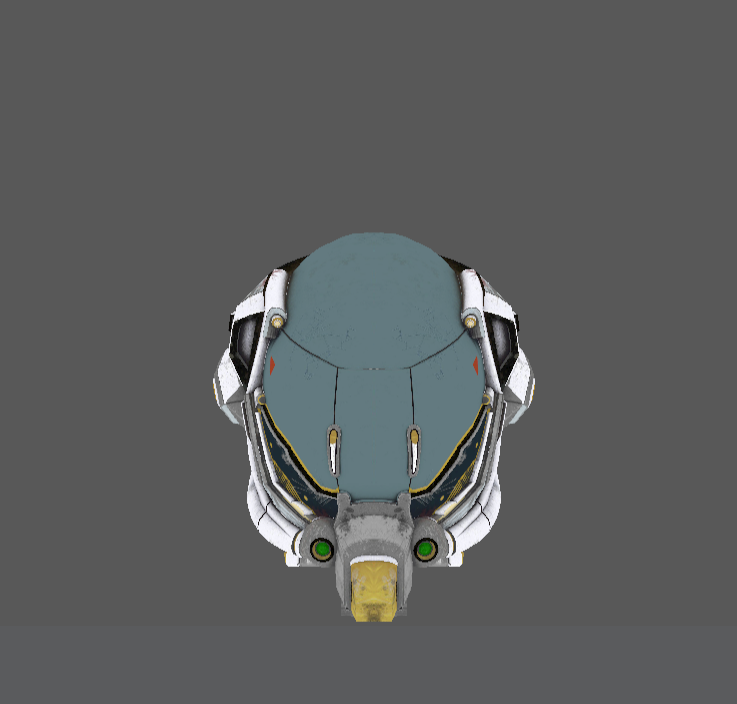
\includegraphics[width=\textwidth]{figures/chapter5/gbuffer-albedo.png}
        \caption*{(a) 反照率 (Albedo)}
    \end{minipage}
    \hfill
    \begin{minipage}{0.48\textwidth}
        \centering
        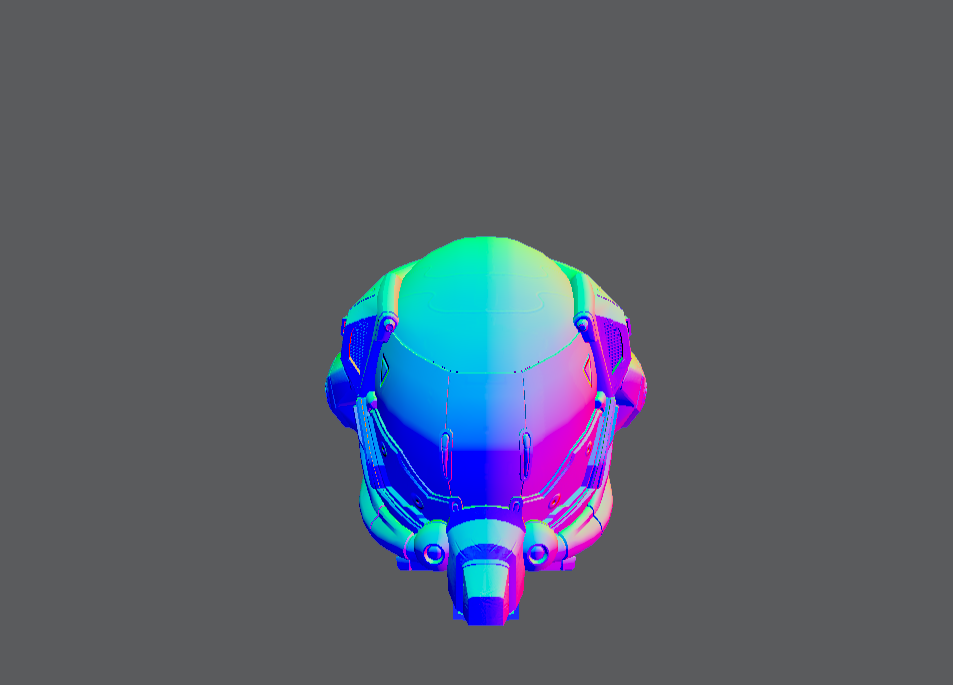
\includegraphics[width=\textwidth]{figures/chapter5/gbuffer-normal.png}
        \caption*{(b) 世界空间法线 (Normal)}
    \end{minipage}
    \vspace{10pt}
    \begin{minipage}{0.48\textwidth}
        \centering
        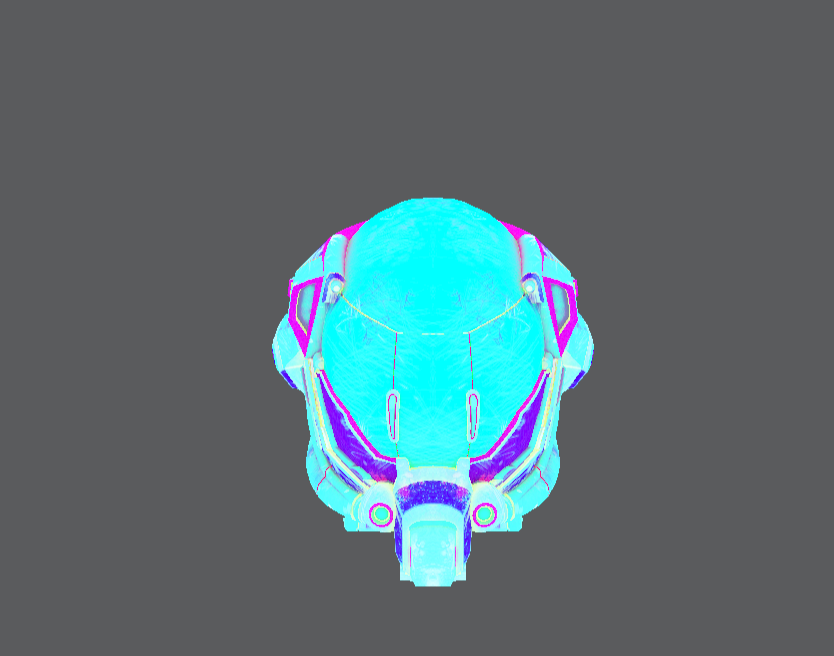
\includegraphics[width=\textwidth]{figures/chapter5/gbuffer-material.png}
        \caption*{(c) 材质属性 (Material)}
    \end{minipage}
    \hfill
    \begin{minipage}{0.48\textwidth}
        \centering
        
\includegraphics[width=\textwidth]{figures/chapter5/gbuffer_depth_linear.png}
        \caption*{(d) 线性深度 (Linear Depth)}
    \end{minipage}
    \caption{混合渲染管线底座：G-Buffer 中间层输出结果}
    \label{fig:gbuffer_outputs_arch}
\end{figure}

\section{架构可视化：基于 Mermaid 的拓扑导出}
为了验证 Render Graph 调度逻辑的正确性，系统集成了拓扑导出功能。通过解析 DAG 中的 Pass 依赖，可以实时生成 Mermaid 格式的流程图，直观展示资源在不同 Pass 间的流转过程。

\section{本章小结}
本章完成了 Chimera 引擎核心调度架构与三大渲染管线的构建。Render Graph 的引入不仅解决了 Vulkan 复杂的同步难题，更为光栅化与光线追踪的深度融合提供了底座。这使得系统能够在下一章中，专注于解决 1 SPP 采样率下的信号重建与画质增强难题。
